\documentclass[11pt, oneside]{amsart}   	% use "amsart" instead of "article" for AMSLaTeX format
\usepackage[margin=1in]{geometry}
\usepackage[]{algorithm2e}
\geometry{letterpaper}
\usepackage{graphicx}
\usepackage{parskip}
\usepackage{amsthm, amsmath, amssymb}

\usepackage{listings}
\usepackage{xcolor}

\usepackage[all]{nowidow}

\definecolor{codegreen}{rgb}{0,0.6,0}
\definecolor{codegray}{rgb}{0.5,0.5,0.5}
\definecolor{codepurple}{rgb}{0.58,0,0.82}
\definecolor{backcolour}{rgb}{0.95,0.95,0.92}

\lstdefinestyle{mystyle}{
    backgroundcolor=\color{white},   
    commentstyle=\color{codegreen},
    keywordstyle=\color{blue},
    numberstyle=\tiny\color{codegray},
    stringstyle=\color{codepurple},
    basicstyle=\ttfamily\footnotesize,
    breakatwhitespace=false,         
    breaklines=true,                 
    captionpos=b,                    
    keepspaces=true,                 
    numbers=right,                    
    numbersep=5pt,                  
    showspaces=false,                
    showstringspaces=false,
    showtabs=false,                  
    tabsize=2
}

\lstset{style=mystyle}

\usepackage[final, colorlinks = true, 
            linkcolor = blue, 
            citecolor = black,
            urlcolor = blue]{hyperref} % For hyperlinks in the PDF

\graphicspath{ {images/} }

\usepackage{datetime2} % Uses YEAR-MONTH-DAY format for dates


%SetFonts
\usepackage{fancyhdr} % Headers and footers

\begin{document}

\title{Homework 4} % Article title
\fancyhead[C]{}
\begin{minipage}{0.295\textwidth} % Left side of title section
\raggedright
CS383: Databases\\ % Your lecture or course
\footnotesize % Authors text size
%\hfill\\ % Uncomment if right minipage has more lines
Isabelle Sanford % Your name
\medskip\hrule
\end{minipage}
\begin{minipage}{0.4\textwidth} % Center of title section
\centering 
\large % Title text size
Homework 4\\ % Assignment title and number
\normalsize % Subtitle text size
Sanderson Elimination Data Stuff \\ % Assignment subtitle
\end{minipage}
\begin{minipage}{0.295\textwidth} % Right side of title section
\raggedleft
\today \\
\footnotesize % Email text size
%\hfill\\ % Uncomment if left minipage has more lines
isanford@brynmawr.edu% Your email
\medskip\hrule
\end{minipage}\\

\section{Database Structure}

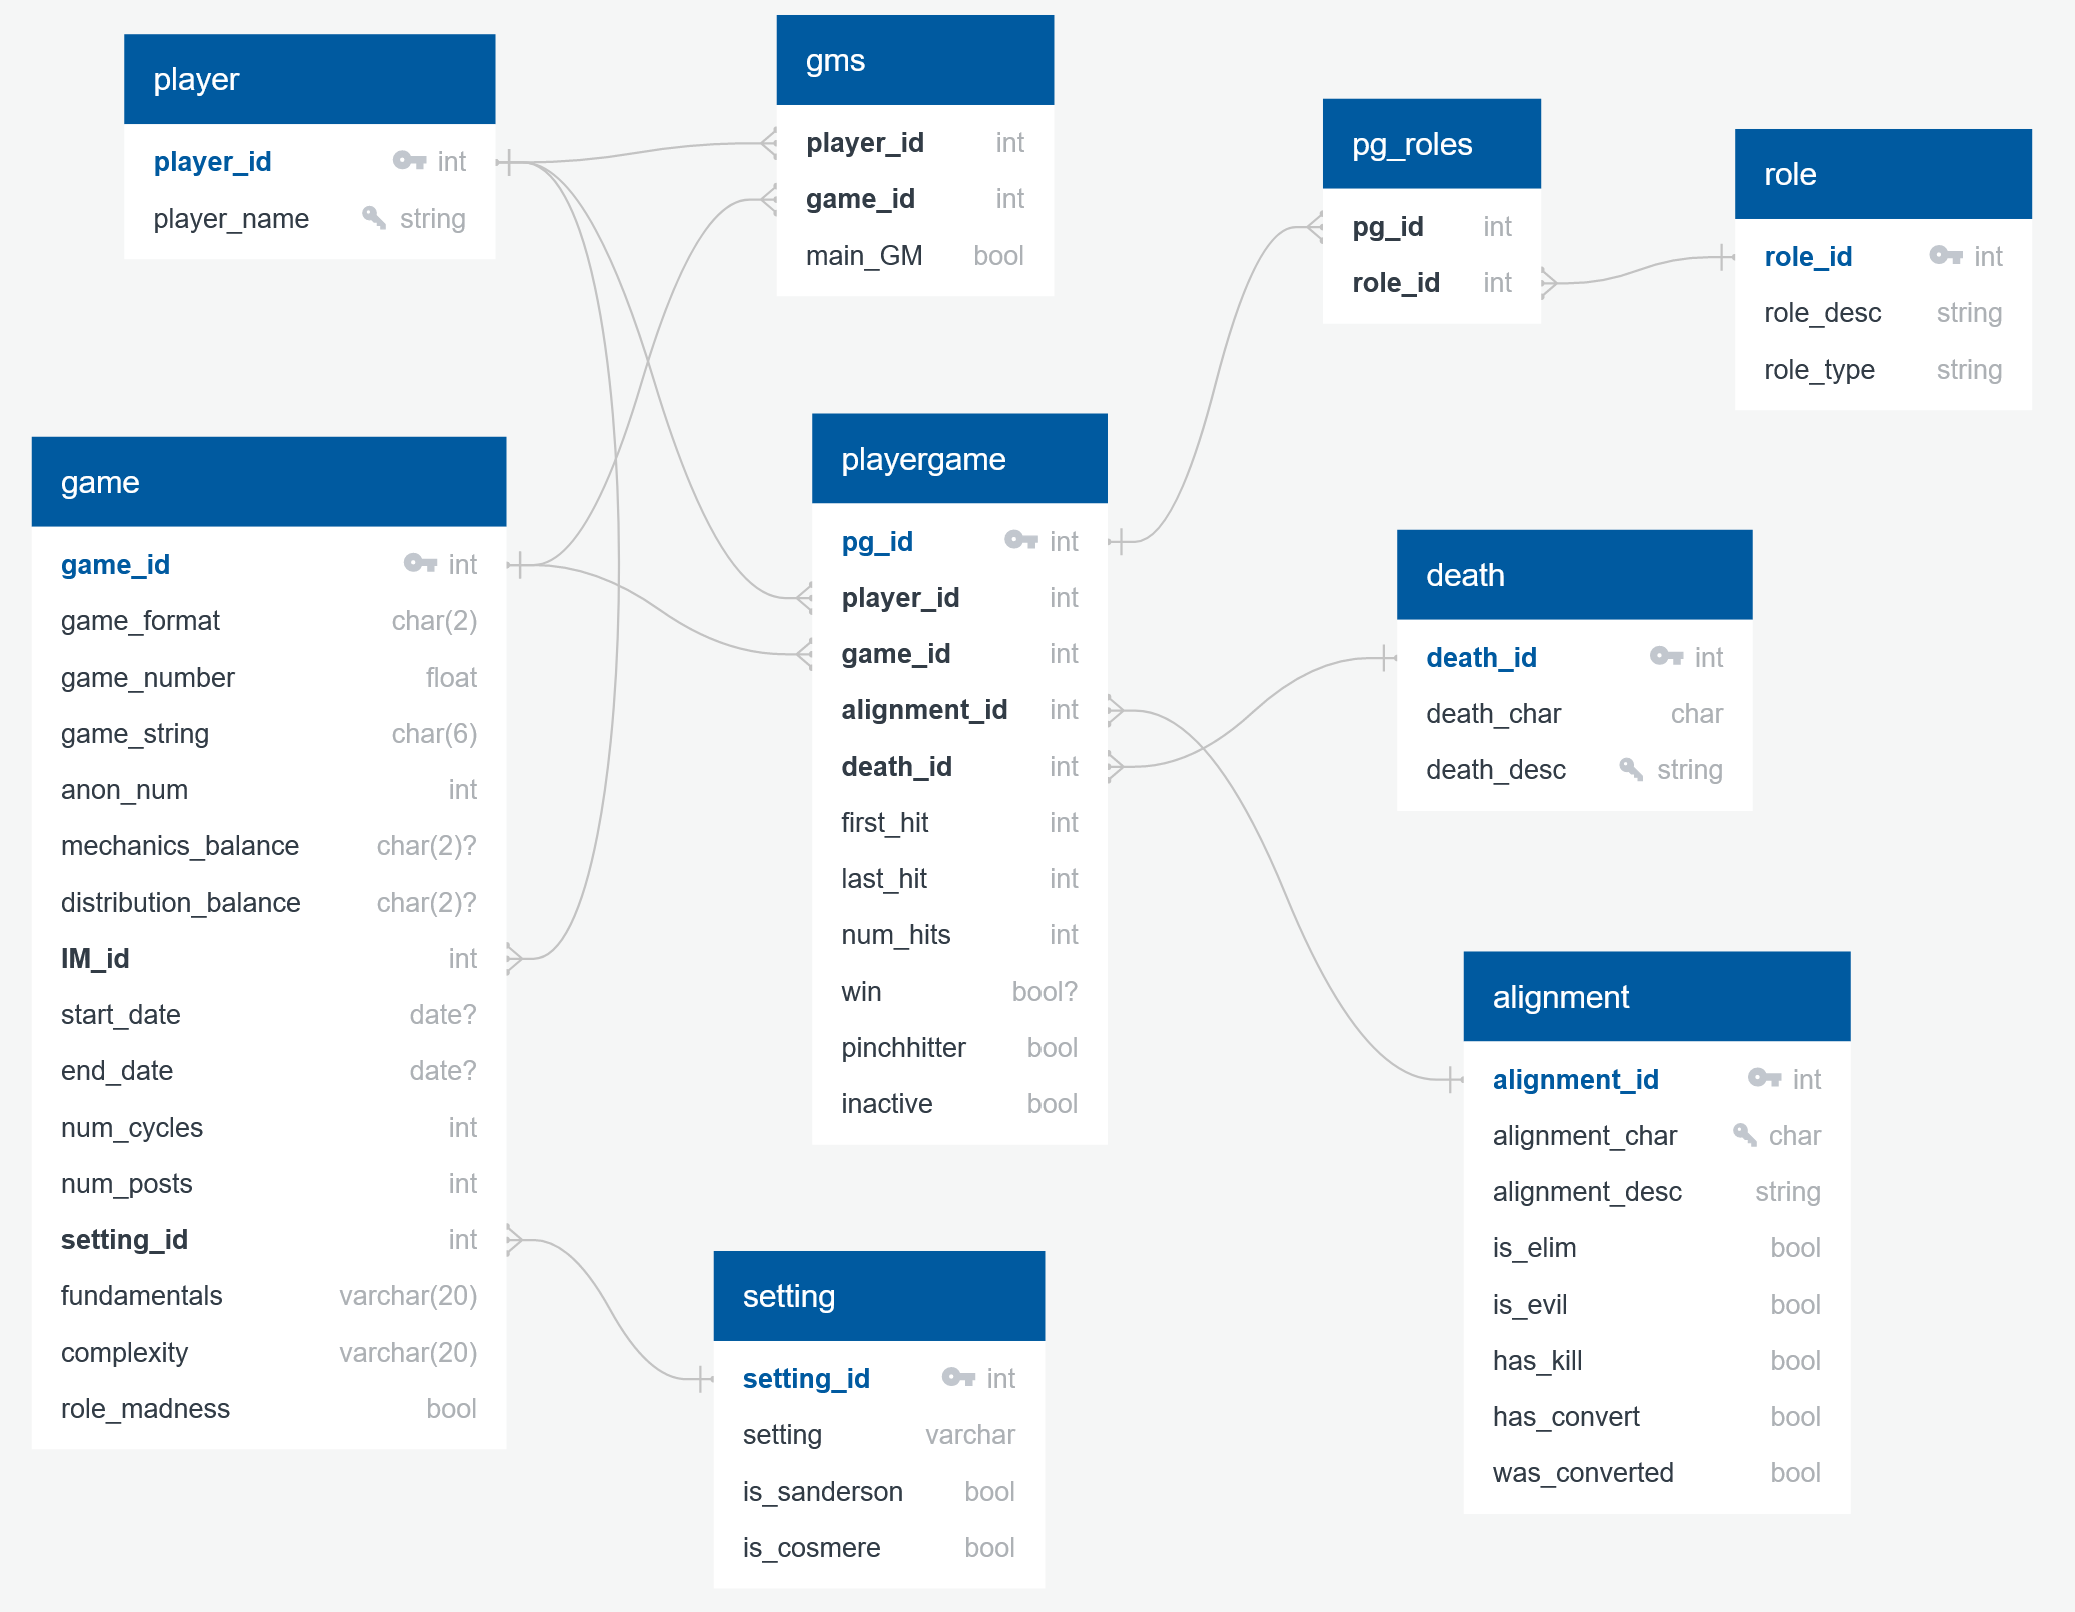
\includegraphics[scale=0.5]{../diagrams/se diagram v3.png}


SIGHHHH

\section{Queries}







\section{univ}

\subsection{Top enrolled courses in CS}

 Find the number of people who have taken each course in the comp sci department. Show only the course name and count. Show only the 2 most commonly taken courses. Sort this list by course name.

\begin{lstlisting}[language=SQL]
with course_counts as 
    (select course_id, count(course_id) as count from takes group by course_id),

top_two as (
    select * from course_counts 
    where course_id in 
        (select course_id from course where dept_name like 'Comp. Sci.')
    order by count desc
    limit 2
)

select title, count
    from top_two natural join course 
    order by title;
\end{lstlisting}

Resulting table: 

\begin{verbatim}
    title                   | count
    ------------------------+-------
    Corporate Law           |   332
    International Practicum |   335
\end{verbatim}

\subsection{Biggest section in fall 2009}

 What section of what course had the most students in fall of 2009?

\begin{lstlisting}[language=SQL]
with thecourse as (select course_id, sec_id, count(sec_id) as c 
    from takes 
    where semester like 'Fall' and year = '2009'
    group by sec_id, course_id
    order by c desc limit 1)

select course_id, sec_id, c, title from thecourse natural join course;
\end{lstlisting}
\textbf{Answer: } Section 1 of course 105 (Image Processing) with 327 students. 

\subsection{3 lowest GPAs}

GPA at this university is defined to be function of the graded earned and the credits for each course. For example suppose, the grades earned in two classes are A and B, and those two classes are worth 2 and 5 credits respectively. Further suppose that A has a value of 4.0 and B has a value of 3.0. Then the GPA calculation is (4.0*2 + 3.0*5)/(2+5)=(8+15)/7=3.29 Show the name, student id and GPA of the three students that have the lowest GPA. 

\begin{lstlisting}[language=SQL]

with creds as (select course_id, credits from course),

takes_creds as (select course_id, id, grade, credits 
    from takes natural join creds), 

takes_pts as (select *, credits*points as cp 
    from takes_creds natural join grade_points),

takes_gpa as (select id, 
    sum(credits) as tot, 
    sum(cp) as totgrad, 
    sum(cp)/sum(credits) as gpa 
    from takes_pts 
    group by id
    order by gpa
    limit 3)

select id, name, gpa from student natural join takes_gpa;

\end{lstlisting}

Table: 
\begin{verbatim}
     id    |  name   |        gpa
    -------+---------+--------------------
     83871 | Stylian | 1.8799999999999997
     507   | Recc    | 1.9823529411764707
     55329 | Vyborny | 2.0565217391304347
\end{verbatim}

\subsection{3 lowest and 3 highest GPAs}

Building from the previous query, in a single table, show the students with the three lowest, and 3 highest, GPAs. Order the resulting table by student name.

\begin{lstlisting}[language=SQL]
    with creds as (select course_id, credits from course),

takes_creds as (select course_id, id, grade, credits 
    from takes natural join creds), 

takes_pts as (select *, credits*points as cp 
    from takes_creds natural join grade_points),

takes_gpa as (select id, 
    sum(credits) as tot, 
    sum(cp) as totgrad, 
    sum(cp)/sum(credits) as gpa 
    from takes_pts 
    group by id), 

gpa_low as (select * from takes_gpa order by gpa limit 3), 
gpa_high as (select * from takes_gpa order by gpa desc limit 3), 
gpa as (select * from gpa_low union select * from gpa_high)

select id, name, gpa
    from gpa natural join student
    order by name;
\end{lstlisting}

Table: 
\begin{verbatim}
     id    |  name   |        gpa
    -------+---------+--------------------
     81207 | Masri   | 3.9904761904761896
     98619 | Nagaraj | 3.9400000000000004
     18286 | Pang    |                3.9
     507   | Recc    | 1.9823529411764707
     83871 | Stylian | 1.8799999999999997
     55329 | Vyborny | 2.0565217391304347
\end{verbatim}

\subsection{Took no classes before 2005}

Find the IDs of students who did not take a class before 2005 (but who have taken a course after 2005). Sort this list by ID and show only the top 5.

\begin{lstlisting}[language=SQL]
    select id
    from takes 
    group by id
    having min(year) > 2004
    order by id
    limit 5;
\end{lstlisting}
(Note: the limit is greater than 2004 there because using 2005 as the lower limit gave exactly 1 student, and the wording is ambiguous.)

Table:
\begin{verbatim}
     id
    -------
     17192
     3163
     33094
     58919
     81550
\end{verbatim}

\subsection{Highest paid instructor whose name starts with A}

Find the name of the instuructor and salary of the highest paid instructor in all departments whose name starts with A.
\begin{lstlisting}[language=SQL]
    select * from instructor where name like 'A%' order by salary desc limit 1;
\end{lstlisting}

\textbf{Answer: } Arias, \$104,563.38 in Statistics. (The wording here arguably means per department, but the only three instructors whose names start with A are all in statistics as far as I can tell. )

\subsection{Lowest salary among highest paid instructors by department}
Find the name of the the instructor, and that person's salary and department, such that they have the highest salary in their department, but a lower salary than that of the highest paid person in any other department.

\begin{lstlisting}[language=SQL]
with ret as (select dept_name, max(salary) as m 
    from instructor 
    group by dept_name 
    order by max(salary)
    limit 1)

select name, salary, ret.dept_name 
    from instructor, ret 
    where instructor.dept_name = ret.dept_name 
        and instructor.salary = ret.m;
\end{lstlisting}
\textbf{Answer: } Soisalon-Soininen, Pyschology, \$62,579.61.


\section{rocket}

\subsection{Max vs All} 
The following two queries both find all launches such that the launch apogee was higher than the launch apogee of any launch in 1957. The first is 15x slower than second!!! Explain.

\begin{lstlisting}[language=SQL]
select apogee, date from launch where apogee > all ( select apogee from launch where date_part('year', date)=1957);

select apogee, date from launch where apogee > ( select max(apogee) from launch where date_part('year', date)=1957);
\end{lstlisting}
            
The former query selects the entire set of 1957 launches, and then compares every row in the table to every single row in that subset (to make sure that the apogee is greater than \textit{all} the 1957 ones). The latter finds the maximum apogee from 1957, and then compares every row in the table to just that single number, which is much faster (roughly by a factor of however many things launched in 1957, though optimization may change that). 

\subsection{Join types}

Consider a query in which you want to join the launch table to the launch\_nonull table on the criteria \texttt{launch\_nonull.mission=launch.mission} and \texttt{launch\_nonull.tag=launch.tag}. Try every variation of join (inner join, natural join, cross join, right outer join, ....). Report the number of rows in the resulting table for each different join. Explain the differences between the sizes of the tables. (You may need to do some other queries to give good explanations.)

\begin{itemize}
    \item Initial table lengths: 72,691 each
    \item Inner: 11,714
    \item Natural: 1,541
    \item Right outer: 72,691
    \item Left outer: 72,691
    \item Full outer: 133,668
    \item Cross: 11,714
\end{itemize}

Natural is so tiny because it joins on every similar column name, which is every single column name, and only retains rows that exactly match, so the result is a table containing only the rows that are identical between the two tables (which seems to be the ones with both a launchpad and mission that are known, i.e. non-null). Inner is joining only on the two specified columns, so if the mission and tag are the same for both tables it includes a union of those rows (which also means several more duplicate columns), so it makes sense that it's somewhat larger than natural join. Right and left outer joins keep all the information from one of the tables and add on information from the other in matching rows, so of course they're the length of whichever table is the outer and then some of the rows now have extra information in other columns. The full outer join joins rows with identical missions and tags but leaves all the other rows from each table in there, which means double the length of the tables ($72691 * 2 = 145382$), minus the number of rows that are joined, which is exactly the number in the inner join ($145382 - 11714 = 133668$ as expected). And then the cross join (so long as you use a where clause) acts exactly like the inner join. (If you don't, you get the full cartesian product, which is $5283981481$. Yikes.)

\section{hurricane}

\subsection{Most recent unnamed storms} Find the first observation of the 5 most recent storms in the database whcih were not given a name (that is, their name is 'UNNAMED').

\begin{lstlisting}[language=SQL]
with lat_date as (select hid, min(date) as min
    from observation 
    where hid in 
        (select hid
            from observation natural join hurricane
            where name like 'UNNAMED'
            group by hid
            order by max(date) desc
            limit 5
        )
    group by hid),

all_obvs as (select observation.*
    from observation join lat_date on true 
    where observation.hid = lat_date.hid
    and observation.date = lat_date.min
    ),

min_times as (select hid, min(time) as mintime
    from all_obvs
    group by hid)

select all_obvs.* from min_times join all_obvs on true 
    where all_obvs.hid = min_times.hid and
    all_obvs.time = min_times.mintime;
\end{lstlisting}
(I apologize for how involved this is and it definitely could be better but it works.)

Table:
\begin{verbatim}
  hid    |    date    |   time   | type | lat  | lathemi | long | longhemi | maxsustained
---------+------------+----------+------+------+---------+------+----------+--------------
AL212005 | 2005-10-04 | 00:00:00 | LO   | 33.8 | N       | 31.8 | W        |       30
AL152013 | 2013-12-03 | 18:00:00 | EX   | 34.3 | N       | 27.7 | W        |       50
AL202011 | 2011-08-31 | 12:00:00 | LO   | 37.1 | N       | 64.3 | W        |       25
AL022006 | 2006-07-16 | 12:00:00 | EX   | 37.2 | N       | 68.7 | W        |       30
AL102004 | 2004-09-07 | 12:00:00 | TD   | 31.5 | N       | 39.7 | W        |       25
\end{verbatim}

\subsection{Longitude negative instead of E}


Write a single query to recreate the observation table where longitude is negative in eastern hemisphere. That is eliminate the longitudehemi column and make any observation in which that column was 'E' have a value in the longitude column that is -1 times the original value.

\begin{lstlisting}[language=SQL]
with eastern as (
    select hid, date, time, type, latitude, latitudehemi, 
        maxsustained, longitude * -1 as newlong
    from observation
    where longitudehemi like 'E'),

western as (
    select hid, date, time, type, latitude, latitudehemi, 
        maxsustained, longitude as newlong
    from observation
    where longitudehemi like 'W')
    
(select * from eastern) union (select * from western);
\end{lstlisting}

Table (start):
\begin{verbatim}
  hid    |    date    |   time   | type | latitude | latitudehemi | maxsustained | newlong
---------+------------+----------+------+----------+--------------+--------------+---------
AL011851 | 1851-06-25 | 00:00:00 | HU   |       28 | N            |           80 |    94.8
AL011851 | 1851-06-25 | 06:00:00 | HU   |       28 | N            |           80 |    95.4
AL011851 | 1851-06-25 | 12:00:00 | HU   |       28 | N            |           80 |      96
AL011851 | 1851-06-25 | 18:00:00 | HU   |     28.1 | N            |           80 |    96.5
AL011851 | 1851-06-25 | 21:00:00 | HU   |     28.2 | N            |           80 |    96.8
AL011851 | 1851-06-26 | 00:00:00 | HU   |     28.2 | N            |           70 |      97
\end{verbatim}


\subsection{Easternmost storm}

Use the answer to the previous question to find the name, date, longitude and latitude of the easternmost observed storm in the database.

\begin{lstlisting}[language=SQL]
with eastern as (
    select hid, date, time, type, latitude, latitudehemi, 
        maxsustained, longitude * -1 as newlong
    from observation
    where longitudehemi like 'E'),

western as (
    select hid, date, time, type, latitude, latitudehemi, 
        maxsustained, longitude as newlong
    from observation
    where longitudehemi like 'W'),
    
un as (select * from eastern union select * from western)

select date, latitude, newlong, name from un natural join hurricane order by newlong limit 1;
\end{lstlisting}

\textbf{Answer: } HOW, October 11 1951, at -63 longitude and 81 latitude.  


\section{null values}
Discuss: null values in a database require ternary logic; which is a pain. So why should you you allow them (give at least two reasons)? What are the alternatives (describe at least one)? Is your alternative to nulls better or worse, why? 

They're useful for a generic non-value that's not specific to individual tables - that is, say I have a table of student grades that range from 0 to 4, and I want to have a value for non-existent. Putting in 0 won't work because that's an actual grade, and putting in even a number outside the range like 100 will mess everything up if I try to take an average. I could put a character like `-' there, but SQL might get unhappy if I tried to do an average then, and I might have to do special logic there. And even if none of that were a problem, someone else might use `NA' or `NaN' or any number of other things where I'd used `-', which is very inconvenient for trying to do anything with multiple tables. So a null value is useful for not interrupting aggregation/math, and for having a systemic not-there value for everyone instead of having everyone make up their own. 

And an alternative is - as noted just above - using specific characters or numbers in place of null, which is way worse because it doesn't necessarily actually avoid ternary logic, it's not standardized across tables, and it's just really annoying to work with. (I guess the other alternative is not allowing nulls, which I think SQL does actually allow you to define column-by-column, and is reasonable if your data is perfectly clean and neat but that is not exactly common.) 




\end{document}


